\paragraph{nonnative-inv}

\subparagraph{Target}
Check the modular inverse relation among three nonnative target objects.

\subparagraph{Constraints logic}
\begin{itemize}
    \item Check equation for gadget: \verb|a * inv_a = 1 + modular * div|.
\end{itemize}

\subparagraph{Process layout}
See \figref{fig:nonnative-inv-layout}.
\begin{figure}[!ht]
    \centering
    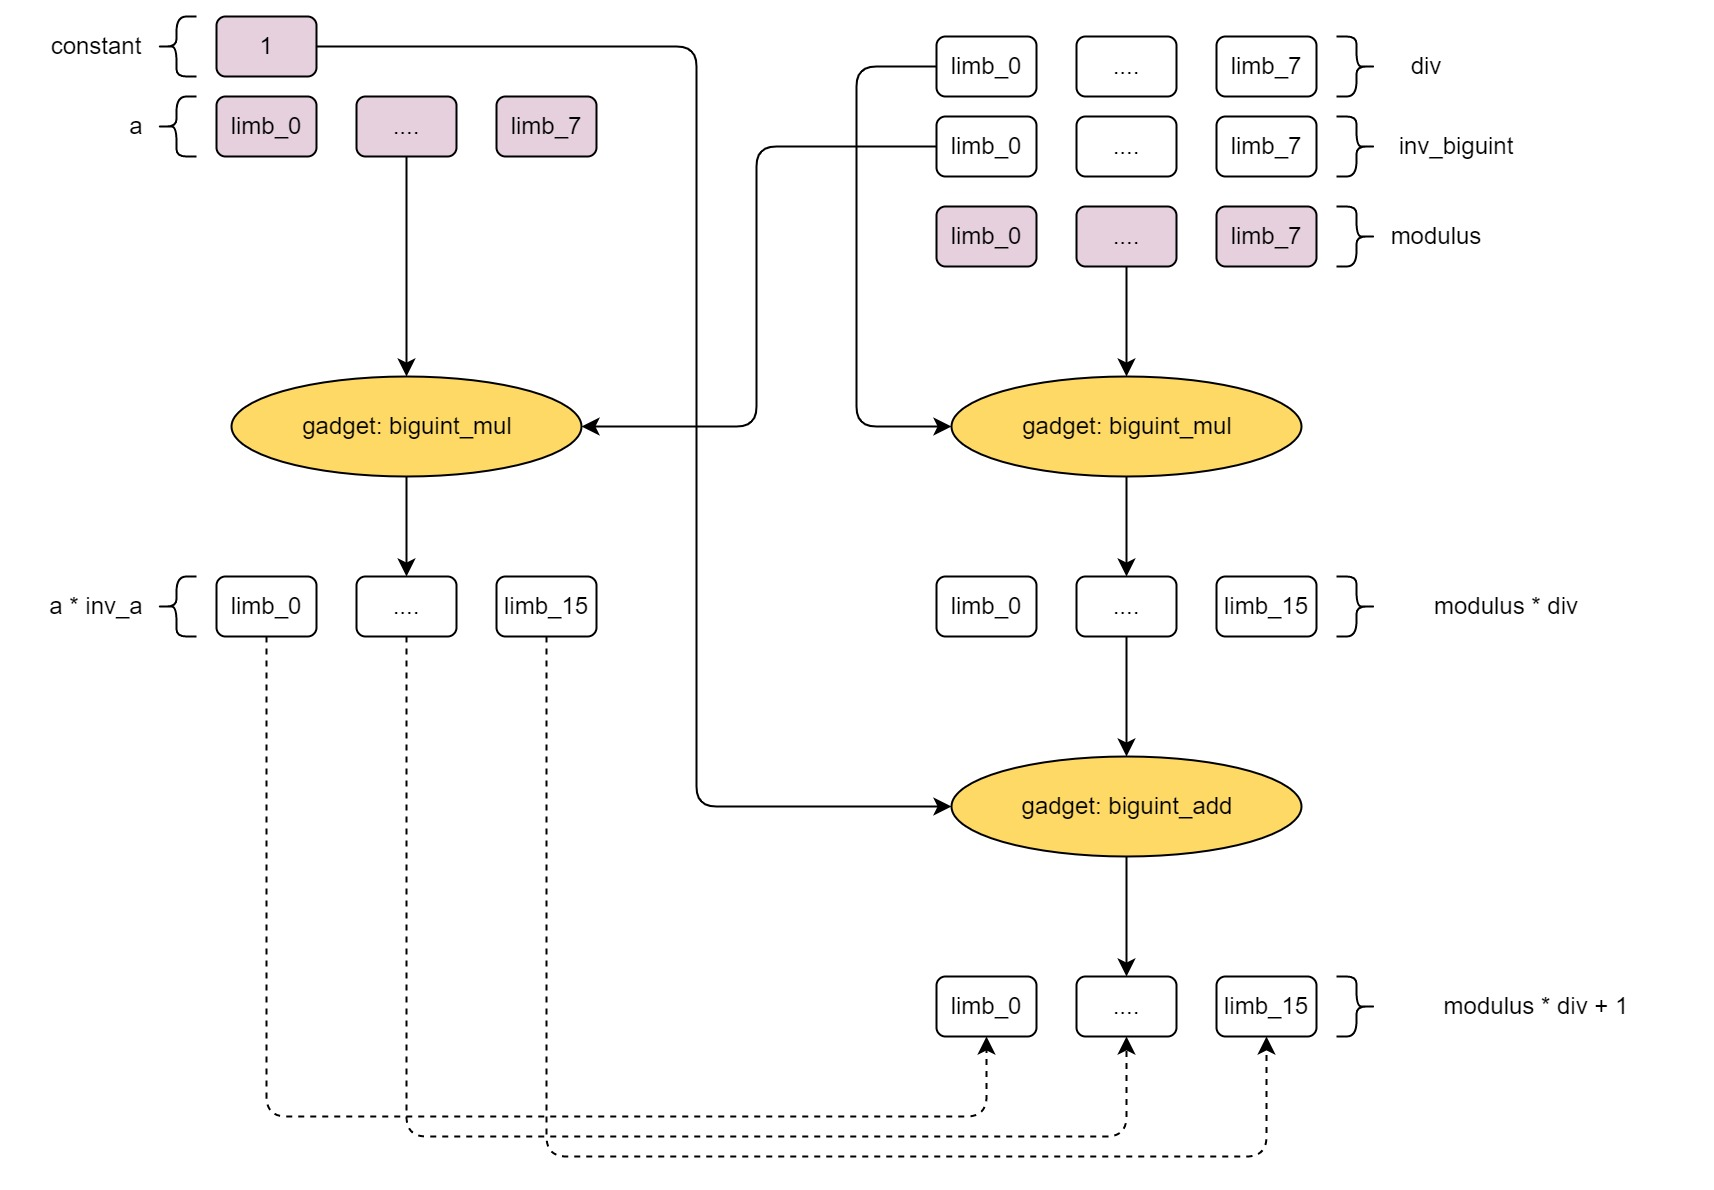
\includegraphics[width=0.6\textwidth]{nonnative-inv-layout.jpg}
    \caption{nonnative-inv layout}
    \label{fig:nonnative-inv-layout}
\end{figure}

\subparagraph{Constraints info and costs}
\begin{itemize}
    \item gadget biguint-add num: 1
    \item gadget biguint-mul num: 2
    \item gate type num: 8 = 7 (U32AddManyGate\{3,5,7,9,11,13,15\}) + 1 (U32ArithmeticGate)
    \item gate instance num: 56 = (8 * 8 + 2) * 2 / 3 + 5 (U32AddManyGate{3}) + 5 + 2 (U32AddManyGate{15})
    \item copy-constraints: 762 = (8 * 8 + 2) * 2 * 3 + 21 * 4 + (6 + 8 + 10 + 12 + 14) * 4 + 4 * 16 + 18
\end{itemize}
